\chapter{Tutorial Pedestrian Lights (Java)}

\section{Scope}

The scope of this tutorial is to demonstrate how to receive model messages from outside the model. Calling 
methods which are not part of the model is simple and you have already done this within the blinky 
tutorial (this is the other way round: model => external code). Receiving events from outside the model is 
a very common problem and a very frequently asked question. Therefore this tutorial shows how an external 
event (outside the model) can be received by the model.

This tutorial is not like hello world or blinky. Being familiar with the basic tool features is mandatory 
for this tutorial. The goal is to understand the mechanism not to learn the tool features.

The idea behind the exercise is, to control a Pedestrian crossing light. We will use the same GUI as for 
the blinky tutorial but now we will use the \textit{REQUEST} button to start a FSM, which controls the 
traffic lights.

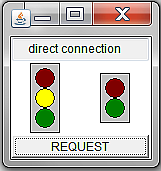
\includegraphics{images/020-Blinky08.png}
% !images/020-Blinky08.png!

The \textit{REQUEST} must lead to a model message which starts the activity of the lights.

There are several possibilities to receive external events (e.g. TCP/UDP Socket, using OS messaging 
mechanism), but the easiest way is, to make a port usable from outside the model. To do that a few steps 
are necessary:
\begin{enumerate}
\item specify the messages (within a protocol) which should be sent into the model
\item model an actor with a port (which uses the specified protocol) and connect the port to the receiver 
\item the external code should know the port (import of the port class)
\item the external code should provide a registration method, so that the actor is able to allow access to 
this port
\item the port can be used from the external code
\end{enumerate}

\section{Setup the model}

\begin{itemize}
\item Use the \textit{New Model Wizzard} to create a new \eTrice{} project and name it 
\textit{PedLightsController}.
\item Copy the package \textit{org.eclipse.etrice.tutorials.PedLightGUI} to your \textit{src} directory 
(see blinky tutorial).
\item In PedestrianLightWndNoTcp.jav uncomment line 15 (import), 36, 122 (usage) and 132-134 
(registration). The error markers will disappear after the code is generated from the model.
\item \begin{flushleft}Copy the model from /org.eclipse.etrice.tutorials/model/PedLightsController to your 
model file, or run the model directly in the tutorial directory.\end{flushleft} 
\item Adapt the import statement to your path.
\end{itemize}

\begin{small}
\begin{verbatim} 
import room.basic.service.timing.* from 
	"../../org.eclipse.etrice.modellib/models/TimingService.room" 
\end{verbatim}
\end{small}

\begin{itemize}
\item Generate the code from the model.
\item Add the org.eclipse.etrice.modellib to the Java Class Path of your project.
\item All error markers should be disappeared and the model should be operable. 
\item Arrange the Structure and the Statemachines to understand the model
\end{itemize}

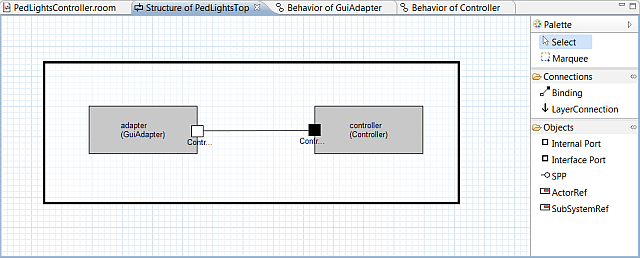
\includegraphics[width=0.8\textwidth]{images/030-PedLights01.png}
% !images/030-PedLights01.png!
The \textit{GuiAdapter} represents the interface to the external code. It registers its 
\textit{ControlPort} by the external code.

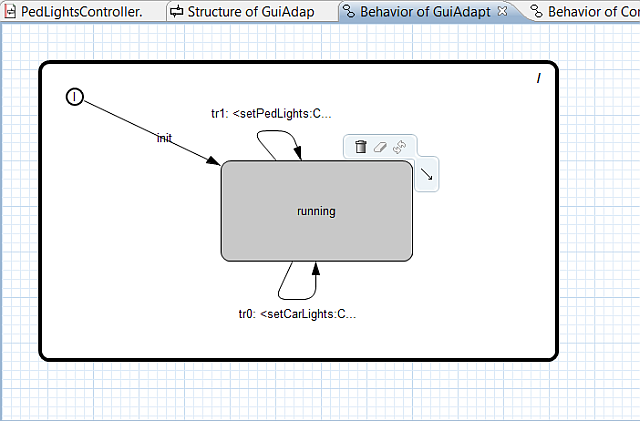
\includegraphics[width=0.8\textwidth]{images/030-PedLights02.png}
% !images/030-PedLights02.png!
Visit the initial transition to understand the registration. The actor handles the incoming messages as 
usual and controls the traffic lights as known from blinky. 

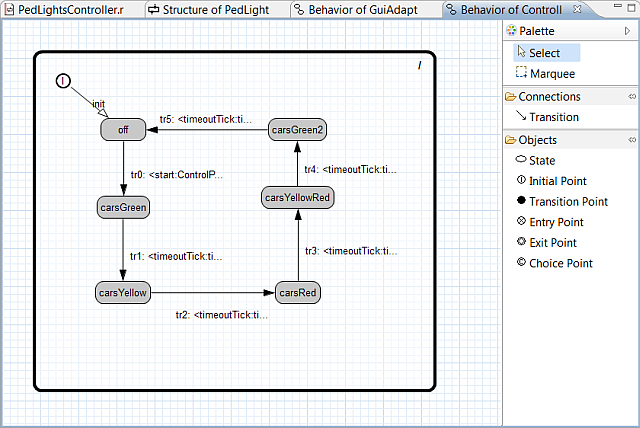
\includegraphics[width=0.8\textwidth]{images/030-PedLights03.png}
% !images/030-PedLights03.png!
The \textit{Controller} receives the \textit{start} message and controls the timing of the lights. Note 
that the \textit{start} message will be sent from the external code whenever the \textit{REQUEST} button 
is pressed.

\begin{itemize}
\item  Visit the model and take a closer look to the following elements:
\begin{enumerate}
\item PedControlProtocol => notice that the start message is defined as usual
\item Initial transition of the \textit{GuiAdapter} => see the registration
\item The \textit{Controller} => notice that the \textit{Controller} receives the external message (not 
the \textit{GuiAdapter}). The \textit{GuiAdapter} just provides its port and handles the incoming messages.
\item Visit the hand written code => see the import statement of the protocol class and the usage of the 
port.
\end{enumerate}
\item Generate and test the model
\item Take a look at the generated MSC => notice that the start message will shown as if the 
\textit{GuiAdapter} had sent it.
\end{itemize}

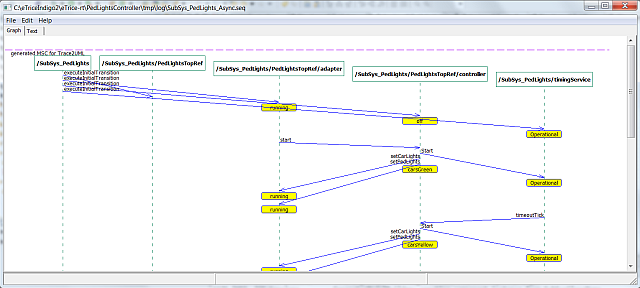
\includegraphics[width=0.8\textwidth]{images/030-PedLights04.png}
% !images/030-PedLights04.png!

\section{Why does it work and why is it safe?}

The tutorial shows that it is generally possible to use every port from outside the model as long as the 
port knows its peer. This is guaranteed by describing protocol and the complete structure (especially the 
bindings) within the model. 
The only remaining question is: Why is it safe and does not violate the \textbf{run to completion} 
semantic. To answer this question, take a look at the \textit{MessageService.java} from the runtime 
environment. There you will find the receive method which puts each message into the queue. 

\begin{verbatim}
    @Override
    public synchronized void receive(Message msg) {
        if (msg!=null) {
            messageQueue.push(msg);
            notifyAll(); // wake up thread to compute message
        }
    }
\end{verbatim}

This method is synchronized. That means, regardless who sends the message, the queue is secured. If we 
later on (e.g. for performance reasons in C/C++) distinguish between internal and external senders (same 
thread or not), care must be taken to use the external (secure) queue.
